\chapter{الحلقات التكرارية (\textenglish{Loops})}

بعدما تعلمنا كيف ننشئ شروطا بلغة 
\textenglish{C}،
سنكتشف معاً 
\textbf{الحلقات التكراريّة} (\textenglish{Loops}).
ما هي الحلقة ؟ هي تقنية تسمح بتكرار نفس التعليمات عدة مرات. و ستساعدنا كثيرا من الآن و صاعدا خاصة في العمل التطبيقي الأوّل الذي ينتظرنا بعد هذا الفصل.

استرخ : هذا الفصل سيكون سهلاً. لقد تعرفنا سابقا على ما تعنيه المتغيّرات المنطقية
(\textenglish{booleans})
و الشروط 
(\textenglish{conditions})
في الفصل السابق، و بذلك كنا قد تخلصنا من عمل كبير. من الآن فصاعداً ستكون الأمور سلسة أكثر و لن يكون في العمل التطبيقي القادم الكثير من المشاكل.

فلننتهز الفرصة، لأننا لن نتأخر في الدخول في الجزء الثاني من الكتاب. سيكون من الجيّد لك أن تنتبه !

\section{ماهي الـحلقة ؟}

كما قلت سابقاً : هي عبارة عن تعليمة تسمح لنا بتكرار نفس التعليمات عدة مرات. 

تماما مثل الشروط، توجد طرق عديدة لإنشاء الحلقات. و لكن مهما اختلفت الطرائق فالهدف واحد : تكرار تعليمات لعدد معيّن من المرات. \\
لدينا في لغة 
\textenglish{C}
ثلاثة أنواع من الحلقات :
\begin{itemize}
	\item \InlineCode{while}
	\item \InlineCode{do \dots while}
	\item \InlineCode{for}
\end{itemize}
في جميع الحالات يبقى المخطط نفسه :

\begin{figure}[H]
	\centering
	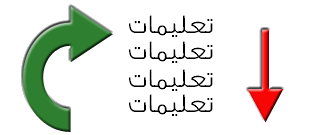
\includegraphics[width=0.4\textwidth]{Chapter_I-7_Loop}
\end{figure}
و هذا ما سيحصل بالترتيب :

\begin{enumerate}
	\item الجهاز يقرأ التعليمات من الأعلى إلى الأسفل كالعادة.
	\item ما إن يصل لنهاية الحلقة يتوجه نحو التعليمة الأولى.
	\item يعيد بعدها قراءة التعليمات كلها من الأعلى إلى الأسفل.
	\item يصل لنهاية الحلقة و يعاود الرجوع للأول من جديد و هكذا \dots
\end{enumerate}

المشكلة في هذا النظام هو أننا إن لم نقم بإيقافه، فالجهاز قادر على تكرار نفس التعليمات إلى مالانهاية ! و لن يتذمّر، أنت تعرف : هو يفعل ما تأمره أنت بفعله \dots يمكنه أن يعلق في حلقة غير منتهية، و هذا النوع من الحالات يعتبر مصدر خوف  بالنسبة للمبرمجين.

و هنا نجد \dots الشروط ! فعندما ننشئ حلقة نقوم دائما بتعريف شرطها. هذا الشرط يعني "كرّر الحلقة دون توقف مادام هذا الشرط صحيحا".

كما قلت، فهناك عدة طرق للقيام بذلك و سنبدأ من دون تأخير بإنشاء حلقة من نوع 
\InlineCode{while}
في الـ\textenglish{C}.

\section{الحلقة \texttt{while}}

هكذا نشكل حلقة 
\InlineCode{while} :

\begin{Csource}
while (/* Condition */)
{
	// The instructions that we want to repeat
}
\end{Csource}

لا يوجد أبسط من هذا. الكلمة 
\InlineCode{while}
تعني "مادام" ، لذا نقول للجهاز: مادام الشرط صحيحا، كرر التعليمات المتواجدة بين الحاضنتين.

أقترح عليك أن نقوم باختبار بسيط : سنطلب من المستعمل ادخال العدد 47، مادام لم يقم بإدخاله، نطلب منه إعادة إدخاله مجدداً \dots و لن يتوقف البرنامج حتى يقوم المستعمل بإدخال العدد 47 (نعم أعرف، إنه عمل شيطاني) :

\begin{Csource}
int entredNumber = 0;
while (entredNumber != 47)
{
	printf("Enter the number 47 ! ");
	scanf("%d", &entredNumber);
}
\end{Csource}

أنظر إلى الاختبار الذي قمت به، للعلم أنني تعمدت الخطأ ثلاث مرات :

\begin{Console}
Enter the number 47 ! 10
Enter the number 47 ! 27
Enter the number 47 ! 40
Enter the number 47 ! 47
\end{Console}

يتوقف البرنامج بعد إدخال العدد 47.\\
 هذه الحلقة 
\InlineCode{while}
 ستتكرر مادام المستعمل لم يدخل العدد 47، لا يوجد أسهل من هذا.
 
الآن لنجعل الأمر ممتعاً أكثر : نريد من الحلقة أن تتوقف بعد عدد معين من التكرارات.\\
لهذا سنستعين بمتغير
\InlineCode{counter}
الذي سيأخذ القيمة $ 0 $ في بداية البرنامج ثم نقوم 
\textbf{بزيادته}،
 هل تتذكر ما قلناه في الفصل السابق حول الزيادة 
(\textenglish{incrementation}) ؟
 التي تنص على إضافة 1 لمتغير حينما نكتب
\InlineCode{variable++}.

إقرأ جيدا الشفرة المصدرية التالية و حاول التمعن فيها و فهمها :

\begin{Csource}
int counter = 0;
while (counter < 10)
{
	printf("Hello !\n");
	counter++;
}
\end{Csource}

النتيجة :

\begin{Console}
Hello !
Hello !
Hello !
Hello !
Hello !
Hello !
Hello !
Hello !
Hello !
Hello !
\end{Console}

البرنامج يكرر عشر مرات العبارة
"\textenglish{Hello !}"

\begin{question}
كيف يعمل هذا بالتحديد ؟
\end{question}

\begin{enumerate}
	\item في البداية لدينا متغير 
	\InlineCode{counter}
	مهيّأ على القيمة الإبتدائية 0.
	\item الحلقة 
	\InlineCode{while}
تأمر بالتكرار مادامت قيمة المتغير
\InlineCode{counter}
أصغر من 10. بما أن قيمة المتغير 
\InlineCode{counter}
هي 0 في البداية، فإننا ندخل في الحلقة لأن الشرط محقق.
	\item نقوم بإظهار الرسالة 
	"\textenglish{Hello !}"
على الشاشة باستخدام الدالة 
\InlineCode{printf}.
	\item نقوم بزيادة قيمة المتغير 
	\InlineCode{counter}
بفضل التعليمة 
	\InlineCode{counter++;}.
كان المتغير
\InlineCode{counter}
يحمل القيمة 0، أمّا الآن فهو يحمل القيمة 1.
	\item نصل لنهاية الحلقة (حاضنة الإغلاق) : نعيد العملية من جديد و نتأكد ما إن كان الشرط محققاً أي ما إن كانت قيمة المتغير أصغر من 10 ؟ في هذه الحالة نعم لأن المتغير
	\InlineCode{counter}
	يحمل القيمة 1 و هي أصغر من 10 إذا سنمرّ بنفس التعليمة داخل الحاضنتين.
\end{enumerate}

و هكذا دواليك،
\InlineCode{counter}
تصبح 1، 2، 3، \dots، 8، 9 ثمّ 10. حينها يصيح الشرط 
\InlineCode{counter < 10}
غير محقق، و عندها نخرج من الحلقة.

و يمكننا ملاحظة أن قيمة المتغير
\InlineCode{counter}
 تزيد في كلّ مرة بواحد. يمكننا التأكّد بـ\InlineCode{printf}~:

\begin{Csource}
int counter = 0;
while (counter < 10)
{
	printf("counter = %d\n", counter);
	counter++;
}
\end{Csource}

\begin{Console}
counter = 0
counter = 1
counter = 2
counter = 3
counter = 4
counter = 5
counter = 6
counter = 7
counter = 8
counter = 9
\end{Console}

إن كنت قد فهمت المثال السابق فقد فهمت كلّ شيء !\\
يمكنك الاستمتاع بتجربة أعداد أكبر من 10 ( مثلا 100 أو أي عدد آخر). كان هذا سيفيدني كثيرا في صغري لكتابة العقوبات الّتي كان يجب عليّ تكرارها مائة مرّة.

\subsection{احذر من الحلقات غير المنتهية ! }

عندما تنشئ حلقة فـ\textbf{تأكّد دائما من جعلها قادرة على التوقف في لحظة معينة !}
إن كان الشرط محققاً دائماً، فلن يتوقف البرنامج أبداً ! و هذا مثال على حلقة غير منتهية :

\begin{Csource}
while (1)
{
	printf("Infinite loop\n");
}
\end{Csource}

تذكر ما قلناه بخصوص القيم المنطقية 
(\textenglish{booleans}) :
فصحيح = 1 و خاطئ = 0. هنا، الشرط محقق دائماً و بهذا فإن البرنامج سيستمرّ في كتابة العبارة 
"\textenglish{Infinite loop}"
بدون توقّف !

\begin{information}
لإيقاف برنامج كهذا في الويندوز، ليس هناك حلّ سوى الضغط على الزر 
\InlineCode{X}
الملوّن بالأحمر في أعلى النافذة بينما على مستخدمي اللينكس الضغط على
\InlineCode{Ctrl} + \InlineCode{C}
للخروج من البرنامج.
\end{information}
\textbf{\textbf{\textbf{}}}
لكن توخ الحذر. تجنب دائما الوقوع في الحلقات غير المنتهية، بالرغم من أنها قد تكون مفيدة في بعض الحالات، خصوصا في برمجة ألعاب الفيديو، هذا ما سنراه لاحقاً.

\section{الحلقة \LR{\texttt{do \dots while}}}

هذا النوع من الحلقات يشبه كثيرا 
\InlineCode{while}
إلا أنه قليل الاستعمال عادة.\\
الشيء الوحيد الذي يتغيّر هو مكان الشرط في الحلقة. فعِوَض أن يكون الشرط في بداية الحلقة، فهو موجود في نهايتها :

\begin{Csource}
int counter = 0;
do
{
	printf("Hello !\n");
	counter++;
} while (counter < 10);
\end{Csource}

ما الذي تغير ؟\\
هذا أمر بسيط فالحلقة 
\InlineCode{while}
يمكن أن لا يتم تشغيلها أبداً إذا كان الشرط غير محقق منذ البداية. فمثلا لو وضعنا القيمة 50 كقيمة ابتدائية للمتغير 
\InlineCode{counter}
فإن الشرط لن يكون محققاً و لذلك لا ندخل في الحلقة أبدا.\\
بالنسبة للحلقة 
\InlineCode{do  \dots while}
فالأمر مختلف : هذه الحلقة تتكرر على الأقل مرة واحدة. في الواقع، اختبار الشرط يتم في نهاية الحلقة كما يمكنك الملاحظة. فلو أعطينا القيمة الإبتدائية 50 للمتغير 
\InlineCode{counter}
فإن التعليمة بين الحاضنتين سيتم تشغيلها مرة واحدة. 

لهذا يجب أحيانا استخدام الحلقات من هذا النوع، لنضمن تكرارها للعملية على الأقل مرة واحدة.

\begin{warning}
هناك استثناء في الحلقة 
\InlineCode{do  \dots while}
يغفل عنه الكثير من المبتدئين، و هو وجود فاصلة منقوطة في نهاية الحلقة ! لا تنس وضع واحدة بعد الـ\InlineCode{while}
و إلا ستظهر لك أخطاء أثناء الترجمة !
\end{warning}

\section{الحلقة \texttt{for}}

نظرياً، الحلقة 
\InlineCode{while}
تلبي رغبتنا في أي نوع كان من التكرارات.\\
سابقا، كما رأينا في الشرط 
\InlineCode{switch}
فإنه توجد أيضا  طريقة أخرى لكتابة حلقة بشكل مختصر أكثر.

الحلقات 
\InlineCode{for}
مستخدمة كثيرا في البرمجة. لا أملك إحصائيات لكن كن واثقاً أنك ستستخدم الحلقة 
\InlineCode{for}
أكثر من الحلقة 
\InlineCode{while}.
و لهذا يجب عليك أن تجيد استخدام كلتا الحلقتين.

و كما قلت لك فالحلقة 
\InlineCode{for}
ماهي إلا عبارة عن طريقة أخرى لكتابة الحلقة
\InlineCode{while}
التي رأيناها قبل قليل.\\
من المثال السابق لدينا :

\begin{Csource}
int counter = 0;
while (counter < 10)
{
	printf("Hello !\n");
	counter++;
}
\end{Csource}

الشفرة المصدرية المكافئة باستعمال الحلقة
\InlineCode{for} :

\begin{Csource}
int counter;
for (counter = 0; counter < 10; counter++)
{
	printf("Hello !\n");
}
\end{Csource}

ما الاختلاف ؟

\begin{itemize}
	\item تلاحظ أننا لم نهيّئ المتغير 
	\InlineCode{counter}
	على قيمة ابتدائية تساوي 0 عند إنشائه (لكنّه كان بإمكاننا فعل ذلك).
	\item هناك الكثير من التفاصيل داخل القوسين بعد 
	\InlineCode{for}،
	سنفصل ذلك لاحقاً.
	\item لا توجد التعليمة 
	\InlineCode{counter++;}
	في الحلقة.
\end{itemize}

فلنهتم بما يوجد بين القوسين فهو كل ما يهم في الحلقة 
\InlineCode{for}.
هناك ثلاث تعليمات مختلفة نفصل فيما بينها بفواصل منقوطة.

\begin{itemize}
	\item الأولى هي
	\textbf{التهيئة}
	(\textenglish{initialisation}) :
	هذه التعليمة تعمل على تحضير المتغير
	\InlineCode{counter}.
	في حالتنا، تهيئته بالقيمة 0.
	\item الثانية هي
	\textbf{الشرط}
	(\textenglish{condition}) :
	كما رأينا في الحلقة 
	\InlineCode{while}
	فإن الشرط يخبرنا ما إن كان يجب تكرار الحلقة أم لا. مادام الشرط محققاً فإن الحلقة تستمر في تكرار التعليمات.
	\item أخيرا،
	\textbf{الزيادة}
	(\textenglish{incrementation}) :
	هذه التعليمة يتم تنفيذها بعد كل التعليمات أي في نهاية الدورة الواحدة و هي تقوم بتعديل قيمة المتغير 
	\InlineCode{counter}
	في كلّ مرة. في غالب الأحيان نقوم بالزيادة، لكن يمكننا أن نستعمل الإنقاص (مثلا 
	\InlineCode{counter{-}{-}})،
	كما يمكننا القيام بعمليّات أخرى، مثلا زيادة قيمة العداد بـ2
	(\InlineCode{counter+=2}).
\end{itemize}

في النهاية، نلاحظ أن حلقة
\InlineCode{for}
ماهي سوى حلقة كتابة مختصرة. تعلّم كيفية استعمالها لأنك ستحتاجها بكثرة !

\section*{ملخّص}

\begin{itemize}
	\item الحلقات هي تعليمات تسمح لنا بتكرار سلسسلة من التعليمات عدة مرات.
	\item توجد كثير من الحلقات :
	\InlineCode{while}،
	\InlineCode{for}
	و 
	\InlineCode{do \dots while}.
	كلّ منها  يُستعمل في الحالة الّتي يكون فيها مناسبا أكثر.
	\item الحلقة
	\InlineCode{for}
	هي التي سنستعملها بكثرة في التطبيقات. نقوم فيها غالباً بزيادات أو إنقاصات للمتغيرات.
\end{itemize}
